{\color{red} Arquitecturas de:}
\begin{itemize}
	\item {\color{red}\texttt{3G UMTS}}\\
	El Sistema Universal de Telecomunicaciones Móviles (UMTS=Universal Mobile Telecomunications System) es un sistema celular móvil de tercera generación para redes basado en el estándar GSM. Desarrollado y mantenido por 3GPP (3rd Generation Partnership Project). \\{ }\\
	\textbf{Arquitectura}\\
	A grandes rasgos la arquitectura de UMTS se ve de la siguiente manera:
	\begin{figure}[ht!]
	\centering
	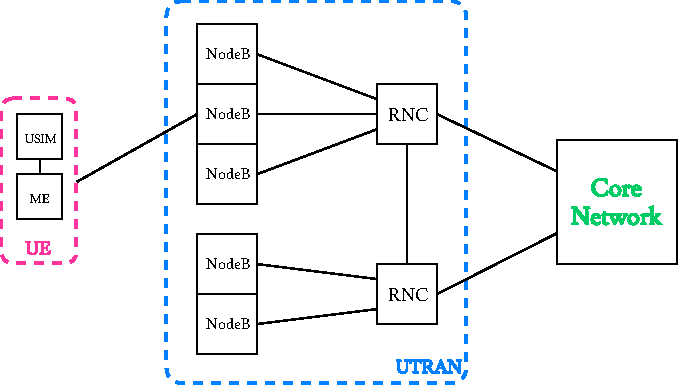
\includegraphics[scale=0.9]{Imagenes/arqUMTS.pdf}
	\end{figure}
	\begin{itemize}
		\item \textbf{UE (User Equipment):} El equipo de usuario o UE es el nombre que se le da al móvil o teléfono celular. También podría ser cualquier cosa entre un teléfono móvil utilizado para hablar con un terminal de datos conectado a una computadora sin capacidad de voz.
			\begin{figure}[ht!]
	\centering
	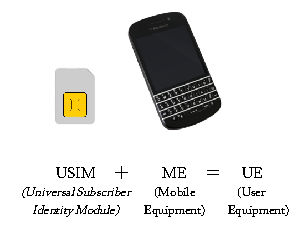
\includegraphics[scale=0.85]{Imagenes/arqUMTS_UE.pdf}
	\end{figure}
		
		
		\item \textbf{UTRAN (UMTS Terrestrial Radio Access Network):} Es un término colectivo para la red y el equipo que conecta teléfonos móviles a la red telefónica pública o Internet. Contiene las estaciones base, que se denominan \textbf{NodeB} y controladores de red de radio (RNC).
	\begin{figure}[ht!]
	\centering
	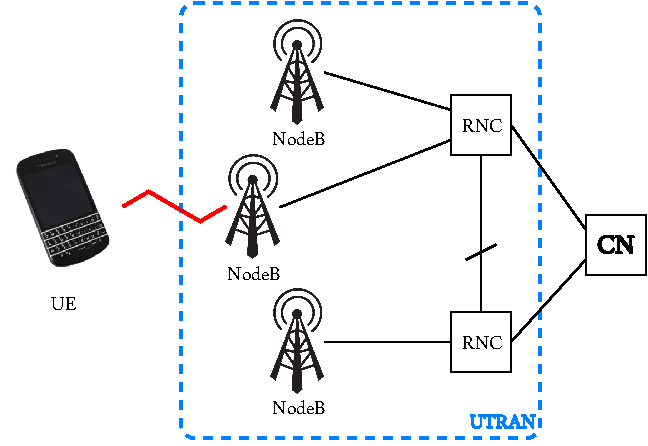
\includegraphics[scale=0.85]{Imagenes/arqUMTS_UTRAN.pdf}
	\end{figure}
	\begin{itemize}
	\item \textbf{RNC (Radio Network Controller):} El RNS también conocido como la red de acceso de radio es el equivalente del BSS en GSM. Proporciona y gestiona la interfaz aérea para la red general.
	\end{itemize}
		\item \textbf{CN (Core Network):} la red principal proporciona todo el procesamiento y la gestión centralizados del sistema.
	\begin{figure}[ht!]
	\centering
	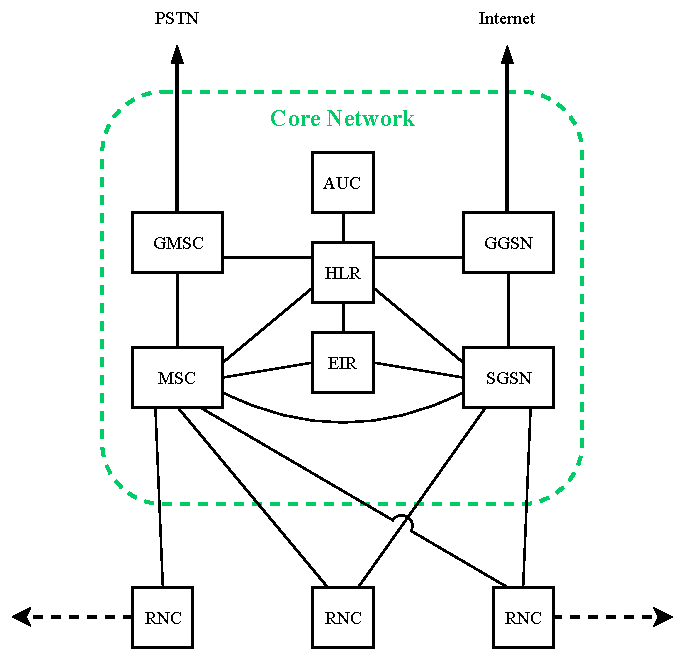
\includegraphics[scale=0.8]{Imagenes/arqUMTS_CN.pdf}
	\end{figure}		
		
		En vista de las diferentes formas en que se pueden transportar los datos, la red central UMTS puede dividirse en dos áreas diferentes: 
		\begin{itemize}
		\item \textbf{Elementos de conmutación de circuitos:} estos elementos se basan principalmente en las entidades de la red GSM y transportan datos de una manera de conmutación de circuitos, es decir, un canal permanente durante la duración de la llamada. \\
		\begin{itemize}
			\item \textbf{Mobile switching centre (MSC):} Este es esencialmente el mismo que el de GSM y gestiona las llamadas conmutadas de circuitos en curso.
			\item \textbf{Gateway MSC (GMSC):} Interfaz para redes externas.\\
		\end{itemize}				
		
		\item \textbf{Elementos de paquetes conmutados:} estas entidades de red están diseñadas para transportar paquetes de datos. Esto permite un uso de la red mucho mayor, ya que la capacidad se puede compartir y los datos se transportan como paquetes que se enrutan de acuerdo con su destino. \\
		\begin{itemize}
		\item \textbf{Serving GPRS Support Node (SGSN):} Como su nombre lo indica, este componente se desarrolló por primera vez cuando se introdujo GPRS y su uso se ha trasladado a la arquitectura de red UMTS. El SGSN proporciona una serie de funciones dentro de la arquitectura de red UMTS. \\
		\begin{enumerate}
		\item \textbf{Gestión de la movilidad:} cuando un UE se conecta al dominio de paquetes conmutados de la red central de UMTS, el SGSN genera información MM\footnote{Mobility Management} basada en la ubicación actual del móvil.
		\item \textbf{Gestión de sesiones:} el SGSN gestiona las sesiones de datos proporcionando la QoS requerida.
		\item \textbf{Interacción con otras áreas de la red:} El SGSN es capaz de administrar sus elementos dentro de la red solo comunicándose con otras áreas de la red.
		\item \textbf{Facturación:} El SGSN también es responsable de la facturación. Lo logra al monitorear el flujo de datos del usuario a través de la red.
		\end{enumerate}
		\end{itemize}
		\item \textbf{Gateway GPRS Support Node (GGSN):} es el elemento central dentro de la red de conmutación de paquetes UMTS. Maneja el interfuncionamiento entre la red conmutada de paquetes UMTS y las redes conmutadas de paquetes externas, y puede considerarse como un enrutador muy sofisticado. En funcionamiento, cuando el GGSN recibe datos dirigidos a un usuario específico, comprueba si el usuario está activo y luego reenvía los datos al SGSN que sirve al UE particular.
		\end{itemize}
	\end{itemize}
	\textbf{Elementos Compartidos}
	\begin{itemize}
	\item \textbf{Home location register (HLR):} Esta base de datos contiene toda la información administrativa sobre cada suscriptor junto con su última ubicación conocida. De esta manera, la red UMTS puede enrutar llamadas al RNC/NodeB correspondiente.
	\item \textbf{Authentication centre (AuC): } es una base de datos protegida que contiene la clave secreta que también se encuentra en la tarjeta USIM del usuario. 
	\item \textbf{Equipment identity register (EIR):}   El EIR es la entidad que decide si un equipo UE dado puede entrar en la red. Cada equipo UE tiene un número conocido como \textit{International Mobile Equipment Identity} (IMEI). Este número está instalado en el equipo y es verificado por la red durante el registro.
	\end{itemize}
	
	\item {\color{red}\texttt{3.5G}} \\
	De acuerdo a la lectura utilizada para la tarea, 3.5G es UMTS con algo llamado High Speed Packet Access (HSPA). 3G UMTS se actualizó con acceso a paquetes de alta velocidad (HSPA) para proporcionar un gran salto en el rendimiento y hacerlo adecuado para cubrir sus requisitos. Los usuarios requerían velocidades mayores que las que podían proporcionar las redes UMTS originales. En consecuencia, los cambios requeridos para HSPA se incorporaron en muchas redes UMTS para permitirles operar más de la manera requerida para las aplicaciones actuales. \\
	
	\textbf{Componentes}\\
	Hay dos componentes principales para 3G UMTS HSPA, cada uno de los cuales se dirige a uno de los enlaces entre la estación base y el equipo de usuario, es decir, uno para el enlace ascendente y otro para el enlace descendente.
	
		\begin{figure}[ht!]
	\centering
	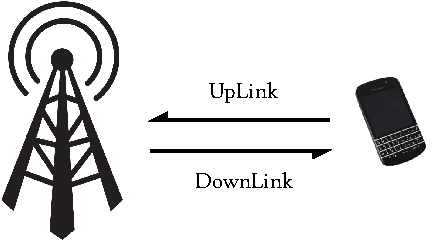
\includegraphics[scale=0.7]{Imagenes/arqUMTS_35.pdf}
	\end{figure}	
	
\begin{itemize}
\item \textbf{High Speed Downlink Packet Access (HSDPA):} Brinda compatibilidad con paquetes de datos, retrasos reducidos y una velocidad máxima de datos sin procesar (es decir, por aire) de 14 Mbps. También proporciona alrededor de tres veces la capacidad de la tecnología 3G UMTS del estándar 3GPP UMTS. 
\item \textbf{High Speed Uplink Packet Access (HSUPA):} proporciona soporte mejorado para paquetes de enlace ascendente, retrasos reducidos y una velocidad máxima de datos sin procesar de 5,74 Mbps. Esto da como resultado un aumento de capacidad de aproximadamente el doble que UMTS.
\end{itemize}	
	
	\item {\color{red}\texttt{3.75G}}\\
	Una vez que se trabajó con HSPA básica, se implementaron más evoluciones en forma de Evolved HSPA/HSPA+/HSPA Evolution. A medida que el uso de datos aumentó aún más, HSPA se mejoró en una serie de revisiones para proporcionar lo que se denominó Evolved HSPA, HSPA + o incluso HSPA Evolution. 
	\item {\color{red}\texttt{3.9G}}\\
	Este proyecto se conoce como Long Term Evolution -LTE y utiliza el acceso de multiplexación por división de frecuencia ortogonal OF-DMA que ofrece una velocidad de datos de 170 Mbps para el enlace ascendente y 320 Mbps para el enlace descendente.
	\item {\color{red}\texttt{4G LTE}}\\
	Después de cambiar de 3G a 4G, se dejó de usar la conmutación de circuitos y se pasó a la conmutación de paquetes por completo. Esta fue la mayor innovación en la nueva generación de redes centrales. Esto tiene como objetivo tener conectividad IP entre UE y red.
	
		
		\begin{figure}[ht!]
	\centering
	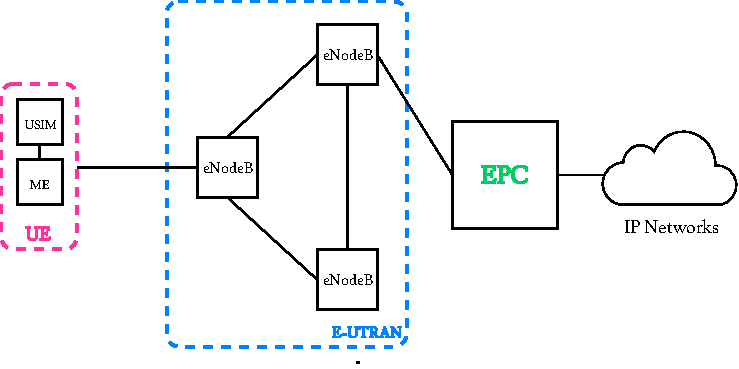
\includegraphics[scale=0.8]{Imagenes/arq4G.pdf}
	\end{figure}	
	\textbf{Componentes}
	\begin{itemize}
	\item \textbf{E-UTRAN (Evolved UMTS Terrestrial Radio Access Network)} \\
	El E-UTRAN maneja las comunicaciones de radio entre el móvil y el EPC y solo tiene un componente, las estaciones base evolucionadas, llamadas \textbf{eNodeB} o eNB. Cada eNB es una estación base que controla los móviles en una o más celdas. La estación base que se comunica con un móvil se conoce como eNB de servicio.
			\begin{figure}[ht!]
	\centering
	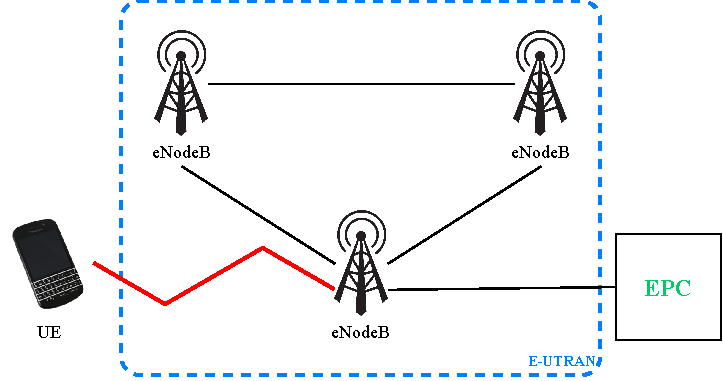
\includegraphics[scale=0.8]{Imagenes/arq4GEUTRAN.pdf}
	\end{figure}
   EL UE LTE se comunica con solo una estación base y una celda a la vez y hay dos funciones principales compatibles con eNB:
   \begin{itemize}
   \item El eBN envía y recibe transmisiones de radio a todos los móviles utilizando las funciones de procesamiento de señales analógicas y digitales de la interfaz aérea LTE.
   \item El eNB controla el funcionamiento de bajo nivel de todos sus móviles, enviándoles mensajes de señalización como comandos de traspaso.\\
   \end{itemize}
	 \item \textbf{EPC (Evolved Packet Core):}\\
   EPC fue introducido por primera vez por 3GPP en la versión 8 del estándar. El EPC representa el núcleo de una red LTE. Está formado por múltiples nodos. Estos nodos ofrecen múltiples funcionalidades como gestión de movilidad, autenticación, gestión de sesiones, configuración de portadores y aplicación de diferentes QoSs.
	\begin{figure}[ht!]
	\centering
	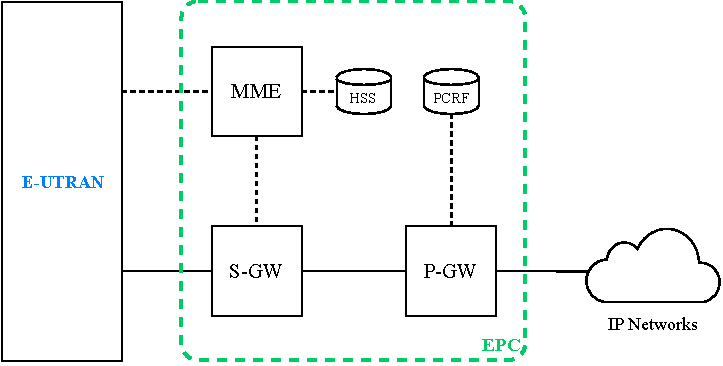
\includegraphics[scale=0.8]{Imagenes/arq4GEPC.pdf}
	\end{figure}		
		
	\end{itemize}
	\begin{itemize}
	\item \textbf{Home Subscriber Server (HSS):} Se encarga de almacenar los datos para el perfil del cliente y crea vectores de autenticación que se envían a MME.
	\item \textbf{Packet Data Network (PDN) Gateway (P-GW):} Una de las principales responsabilidades de P-GW es asignar la IP al UE. Es responsable del filtrado de los paquetes IP de usuario de enlace descendente en los diferentes portadores basados en QoS.
	\item \textbf{Serving Gateway (S-GW):} Es responsable de intercambiar el tráfico entre P-GW y 4G E-UTRAN. Los paquetes IP que provienen del usuario se pasan desde S-GW. Es como un ancla de movilidad local para los portadores de datos cuando UE cambia los eNodeB. Además de esto, S-GW es responsable de algunas funciones administrativas, como recopilar información sobre la facturación de las redes.
	\item \textbf{Mobility Management Entity (MME):} Es responsable de proporcionar la gestión de Movilidad y Sesión a los Equipos de Usuario. Es el nodo de control que gestiona la señalización entre UE y el Core Network.
	\item \textbf{Policy Control and Charging Rules Function (PCRF):} Es responsable de proporcionar la información de QoS a P-GW. Esta información puede incluir reglas de tarificación, reglas de control de flujo y prioridad del tráfico.
	\end{itemize}

	\item {\color{red}\texttt{5G}}\\
	5G es la quinta generación de redes móviles, una evolución significativa de las redes 4G LTE actuales. 5G ha sido diseñado para satisfacer el gran crecimiento de datos y conectividad de la sociedad moderna de hoy, el Internet de las cosas con miles de millones de dispositivos conectados. 5G operará inicialmente junto con las redes 4G existentes antes de evolucionar a redes totalmente independientes en versiones posteriores y expansiones de cobertura.
		\begin{figure}[ht!]
	\centering
	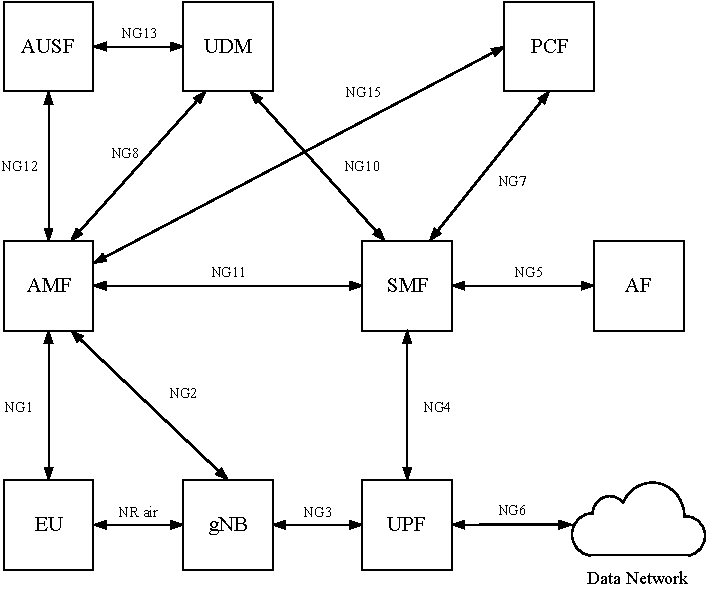
\includegraphics[scale=0.8]{Imagenes/arq5G.pdf}
	\end{figure}\\
	\textbf{Componentes}
	\begin{itemize}
	\item \textbf{Access and Mobility Management Function (AMF):} Cifrado NAS y protección de integridad, administración de registros, administración de conexiones, administración de movilidad, autenticación y autorización de acceso, contexto de seguridad.
	\item \textbf{User Plane Dunction (UPF):} enrutamiento y reenvío de paquetes, inspección de paquetes, manejo de QoS.
	\item \textbf{Session Management Function (SMF):} Asigna direcciones IP a UE, envía QoS e información de políticas a RAN a través de AMF, notificación de datos de enlace descendente y actúa como interfaz para todas las comunicaciones relacionadas con los servicios de plano de usuario ofrecidos. SMF determina cómo se aplica la política y el cobro por estos servicios.
	\item  \textbf{Policy Control Function (PCF):} El 5G PCF realiza la misma función que el PCRF en redes 4G. Proporciona reglas de política para las funciones del plano de control. Esto incluye la división de redes, la itinerancia y la gestión de la movilidad.
	\item \textbf{Authentication Server Function (AUSF):} El AUSF realiza la función de autenticación de 4G HSS.
	\item \textbf{Unified Data Management (UMD):} El UDM realiza partes de la función 4G HSS como: Generación de credenciales de Autenticación y Acuerdo de Clave, Identificación de usuario, Autorización de acceso, Gestión de suscripciones.
	\item \textbf{Application Function (AF):} admite la influencia de la aplicación en el enrutamiento del tráfico.
 	\end{itemize}
\end{itemize}


\begin{thebibliography}{9}
\bibitem{tutorialspoint} 
3G UMTS Network Architecture. \href{https://www.electronics-notes.com/articles/connectivity/3g-umts/network-architecture.php}{https://www.electronics-notes.com/articles/connectivity/3g-umts/network-architecture.php}

\bibitem{ques10} 
Explain UMTS network architecture in detail with interface \href{https://www.ques10.com/p/38287/explain-umts-network-architecture-in-detail-with-i/}{https://www.ques10.com/p/38287/explain-umts-network-architecture-in-detail-with-i/}


\bibitem{3GPP} 
Industry Experience on Multi-Network Deployment.\\ \href{https://www.3gpp.org/component/itpgooglesearch/search?gsquery=3.75G}{https://www.3gpp.org/component/itpgooglesearch/search?gsquery=3.75G} ZTE Corporation.

\bibitem{3g4g} 
3G $\longrightarrow$ 3.9G \href{https://blog.3g4g.co.uk/2007/05/3g-39g.html?m=1}{https://blog.3g4g.co.uk/2007/05/3g-39g.html?m=1} The 3G4G Blog .

\bibitem{3g4g2} 
What is HSPA: Tutorial. \href{https://www.electronics-notes.com/articles/connectivity/3g-hspa/what-is-hspa-high-speed-packet-access-tutorial.php}{https://www.electronics-notes.com/articles/connectivity/3g-hspa/what-is-hspa-high-speed-packet-access-tutorial.php}

\bibitem{3g4g3} 
Evolved HSPA / HSPA+  \href{https://www.electronics-notes.com/articles/connectivity/3g-hspa/evolved-hspa-plus.php}{https://www.electronics-notes.com/articles/connectivity/3g-hspa/evolved-hspa-plus.php}

\bibitem{3g4g4} 
*HSPA+  Nueva y poderosa Tecnología con la mejor RED del Continente  \href{https://www.sites.google.com/site/solucionesiusacell/HSPA}{https://www.sites.google.com/site/solucionesiusacell/HSPA}

\bibitem{3g4g4} 
Differences on 1G 2G 2.5G 3G 3.5G 3.75G 3.9G 4G  \href{https://vctechblog.wordpress.com/2015/10/01/differences-on-1g-2g-2-5g-3g-3-5g-3-75g-3-9g-4g-networks-in-india/}{https://vctechblog.wordpress.com/2015/10/01/differences-on-1g-2g-2-5g-3g-3-5g-3-75g-3-9g-4g-networks-in-india/}

\bibitem{radish} 
LTE Network Architecture  \href{http://rashidtelecom.blogspot.com/2015/11/lte-4g.html}{http://rashidtelecom.blogspot.com/2015/11/lte-4g.html}

\bibitem{medium} 
Evolution of Core Network(3G vs. 4G vs. 5G)  \href{https://medium.com/@sarpkoksal/core-network-evolution-3g-vs-4g-vs-5g-7738267503c7}{https://medium.com/@sarpkoksal/core-network-evolution-3g-vs-4g-vs-5g-7738267503c7}

\bibitem{3gpporg} 
The Evolved Packet Core \href{https://www.3gpp.org/technologies/keywords-acronyms/100-the-evolved-packet-core}{https://www.3gpp.org/technologies/keywords-acronyms/100-the-evolved-packet-core}


\bibitem{yatebts} 
Evolved Packet Core (LTE EPC). \href{https://yatebts.com/solutions\_and\_technology/lte-epc}{https://yatebts.com/solutions\_and\_technology/lte-epc}

\bibitem{emfexplained} 
5G Explained - How 5G Works  \href{http://www.emfexplained.info/?ID=25916}{http://www.emfexplained.info/?ID=25916}

\bibitem{3g4g5g} 
5G Network Architecture and Design Update. \href{https://blog.3g4g.co.uk/2017/02/5g-network-architecture-and-design.html}{https://blog.3g4g.co.uk/2017/02/5g-network-architecture-and-design.html}, 2017.

\bibitem{SBA} 
5G Service-Based Architecture (SBA) \href{https://medium.com/5g-nr/5g-service-based-architecture-sba-47900b0ded0a}{https://medium.com/5g-nr/5g-service-based-architecture-sba-47900b0ded0a}, Octubre, 2018.

\bibitem{SBA} 
5G Reference Network Architecture \href{http://www.techplayon.com/5g-reference-network-architecture/}{http://www.techplayon.com/5g-reference-network-architecture/}.

\end{thebibliography}

